\chapter*{Исполнитель Водолей}
\addtocounter{chapter}{1}


\section{Окна}

При запуске исполнителя создаются два окна (см.~\ref{vodoley}):
\begin{itemize}
\item окно водолея
\item окно пульта
\end{itemize}
\begin{figure}[h]
	\begin{center}
		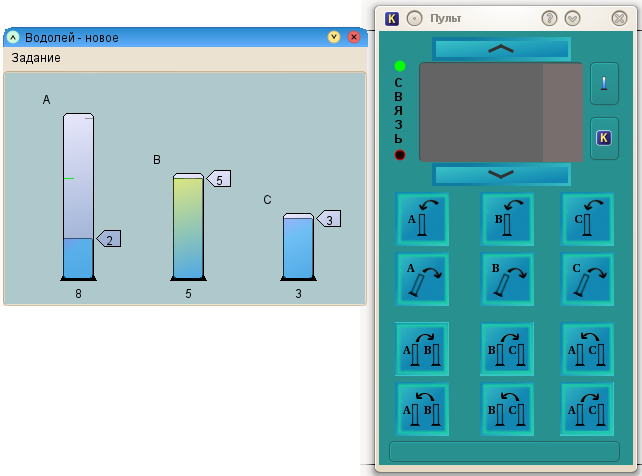
\includegraphics[scale=0.6]{vodoley.png}
	\end{center}
	\caption{Окна Водолея и его пульта. На окне Водолея под каждым стаканом показан его объем, бирки справа от каждого стакана показывают текущий объем воды в нем. В окошке вверху окна (на темно-синем фоне) показано количество воды, которое нужно получить, это же количество отмечено зеленой полоской на каждом из стаканов.}
\label{vodoley}
\end{figure}
Окна пульта и водолея --- стандартные окна операционной системы. Их можно передвигать по экрану, сворачивать и разворачивать обычным образом.Окно водолея можно закрепить поверх всех окон для этого слева на заголовке имеется кнопка.

\emph{Ограничение:} размеры окон менять нельзя.

С точки зрения операционной системы, окно пульта является основным. При попытке его закрыть будет закрыто и окно водолея.

\section{Правила игры. Задание}

Даны три стакана, объем каждого стакана --- целое число ( Стакан С может иметь размер 0. В этом случае он не показывается)

У игрока есть следующие возможности:
\begin{enumerate}
\item долить нужный стакан доверху («из крана»);
\item вылить всю воду из указанного стакана (при этом стакан становится пустым);
\item перелить воду из одного стакана в другой (если удается перелить всю воду, то первый стакан становится пустым; в противном случае второй стакан становится полным, а остаток остается в первом стакане.
\end{enumerate}

\emph{Пример.} Стакан A имеет объем 10 литров, стакан B имеет объем 6 литров; в стакане А находится 7 литров воды, а в стакане B --- 2 литра.  Если перелить воду из стакана B в стакан А, то в стакане А станет 8 литров, а в стакане B --- ничего.   Если перелить воду из стакана А в стакан B, то в стакане А станет 3 литра, а в стакане B --- 6 литров (стакан будет наполнен доверху).

Цель игры --- получить в каком-либо из стаканов указанное количество воды (начальное количество воды в каждом стакане также задано).	Таким образом, \emph{задание} игры Водолей состоит из семи целых чисел:
\begin{enumerate}
\item объемы каждого из стаканов (три числа);
\item начальное количество воды в каждом из стаканов (три числа);
\item требуемое количество воды (одно число).
\end{enumerate}

\section{Окно водолея}

Окно водолея – прямоугольное (см.~\ref{vodoley}). Оно содержит рабочее поле голубого цвета (на нем расположены три сосуда, обозначенные латинскими буквами «A», «B», «C»),  а также верхнюю панель, на котором находится меню «Задание».

Меню «Задание» содержит три пункта:
\begin{itemize}
\item Новое
\item Сохранить
\item Загрузить
\end{itemize}

При выборе пункта «Новое» откроется окно редактирования текущего задания (см.~\ref{vodoley-task}), где можно указать размер каждого стакана, тот уровень, на который стакан уже наполнен в начале работы, и количество воды, которое нужно отмерить (желаемый результат).
\begin{figure}[h]
	\begin{center}
		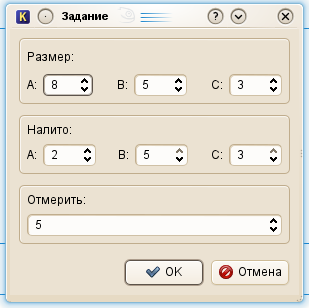
\includegraphics[scale=0.6]{vodoley-task.png}
	\end{center}
	\caption{Установка задания для Водолея}
\label{vodoley-task}
\end{figure}

При выборе пунктов «Сохранить» и «Загрузить» появляются диалоговые окна сохранения и выбора уже готового задании соответственно. При команде «Загрузить»  задание из выбранного файла (текстовый файл с расширением \textsf{.vod}) становится текущим. При этом директория по умолчанию – это директория, которая последней использовалась для операций «Сохранить» и «Загрузить».

В рабочем поле окна Водолея изображены три стакана. Под каждым стаканом указана его емкость, справа на плавающей бирке указано текущее количество воды. Справа на стакане есть риска, обозначающая количество воды, которое требуется получить. В окошке вверху окна (на темно-синем фоне) показано количество воды,  которое нужно получить, это же количество отмечено зеленой полоской на каждом из стаканов. Когда это количество воды будет получено, цвет окошка вверху изменится на зеленый, а цвет воды в стакане, в котором оказалось нужное количество воды --- на золотой.

\section{Окно пульта}

Окно пульта содержит:
\begin{itemize}
\item поле протоколирования команд (бесконечное вниз) и кнопки прокрутки протокола (сверху и снизу от поля);
\item индикатор связи Водолея с пультом --- слева от поля протокола;
\item кнопку сброса (справа от протокола вверху); при нажатии этой кнопки задание Водолея сбрасывается в исходное положение текущего задания, а поле протокола очищается;
\item кнопку передачи протокола в КуМир (справа от протокола внизу); по нажатию этой кнопки содержимое команд протокола вставляется в программу в окне редактирования системы КуМир; 
\item двенадцать кнопок для передачи команд черепахе («наполни А», наполни В», «наполни С», «вылей А», «вылей В», «вылей С», «перелей из А в В», «перелей из В в С», «перелей из С в А», «перелей из В в А», «перелей из С в В», «перелей из~А~в~С»).
\end{itemize}

\subsection{Система команд}

При работе под управлением КуМира Водолей понимает следующие команды:
\textsf{
\begin{itemize}
\item наполни А 
\item наполни B
\item наполни C
\item вылей А
\item вылей B
\item вылей C
\item перелей из A в B
\item перелей из A в C
\item перелей из B в A
\item перелей из B в C
\item перелей из C в A
\item перелей из C в B
\end{itemize}
}